\documentclass[10pt]{article}

\usepackage[a4paper,margin=0.78in]{geometry}
\usepackage{amsmath,amssymb,amsthm,mathtools}
\usepackage{microtype}
\usepackage{booktabs}
\usepackage{tabularx}
\usepackage{enumitem}
\usepackage{xcolor}
\usepackage{tikz}
\usetikzlibrary{arrows.meta,positioning}
\usepackage[colorlinks=true,linkcolor=blue!45!black,
  citecolor=blue!45!black,urlcolor=blue!45!black]{hyperref}

\newtheorem{theorem}{Theorem}
\newtheorem{corollary}[theorem]{Corollary}
\newtheorem{proposition}[theorem]{Proposition}
\theoremstyle{definition}
\newtheorem{definition}[theorem]{Definition}

\newcommand{\Q}{\mathbb Q}
\newcommand{\R}{\mathbb R}
\newcommand{\C}{\mathbb C}
\newcommand{\N}{\mathbb N}
\newcommand{\T}{\mathbb T}
\newcommand{\rank}{\operatorname{rank}}
\newcommand{\spanQ}{\operatorname{span}_{\Q}}
\newcommand{\sinc}{\operatorname{sinc}}

\title{\textbf{A universal law separates quantum recurrence
from spatial localization}}
\author{Michael Haufschild}
\date{31 July 2026}

\begin{document}
\maketitle

\begin{abstract}
Does preventing a quantum system from moving also make its long-term future
simpler? We prove that it need not. Every finite spectrum obeys an exact
conservation law: rational projective gap rank plus exact recurrence-relation
rank equals the number of levels minus one. Walsh duality turns this budget
into a complete classification for diagonal l-bit Hamiltonians. A free
\(N\)-mode Fock spectrum has at most \(N\) recurrence directions, whereas
interactions diagonal in the same product basis can attain all \(2^N-1\)
without moving any configuration. For every finite Hermitian hopping matrix
and every positive spatial envelope, one fixed-hopping Hamiltonian likewise
has maximal projective rank while every off-diagonal transition remains
below the envelope for all time. Conversely, exponential localization of
the spectral weight seen at one site compresses its guaranteed recurrence
deadline to the number of modes in one localization volume, independently
of the ambient spectral dimension; this remains true for countably infinite
pure-point spectra. The infinite interacting law is sharper. One
absolutely summable l-bit field simultaneously obeys the volume-independent
bound
\(\|[\tau_t(X_x),X_y]\|\le\min\{2,4K|t|2^{-|x-y|}\}\)
and has \(2^{|F|}\) independent conditional frequencies for every finite
environment \(F\). Nevertheless, every distinct pair of sites attains the
two-unit commutator ceiling at a positive time \(t_{xy}\), necessarily with
\(2\le4Kt_{xy}2^{-|x-y|}\). Thus influence can be exponentially delayed at
every distance without being permanently extinguished. Adding one boundary
site doubles the exact conditional recurrence dimension from \(D\) to
\(2D\); the same boundary-crossing coefficient packet obeys a locality
budget, and resolving all \(D\) new directions above coefficient threshold
\(\delta\) forces \(2\delta D^2\le K\). Anderson dynamical localization,
which requires spatial decay after taking the supremum over all times, is
therefore mathematically distinct from interacting quasi-local delay.
\end{abstract}

\noindent\textbf{One-sentence summary.}
Localization makes a local quantum history recur by a clock set by its
visible neighborhood rather than the size of the world, while interactions
can still transmit influence across every distance at sufficiently late
times.

\section{A different question about localization}

Anderson localization changed the meaning of disorder in quantum mechanics:
interference can suppress transport rather than produce diffusion
\cite{Anderson1958}. Its interacting descendant, many-body localization,
adds a second phenomenon. Quasi-local conserved degrees of freedom can
remain spatially localized while weak interactions between them generate
dephasing over a hierarchy of time scales
\cite{SerbynPapicAbanin2013,HuseNandkishoreOganesyan2014}. Revivals of local
observables are correspondingly suppressed by interactions
\cite{VasseurParameswaranMoore2015}. Exponentially localized integrals of
motion already imply a logarithmic light cone
\cite{KimChandranAbanin2014}; local l-bit spectra already form exponentially
branching line trees \cite{NandkishoreGopalakrishnanHuse2014}; and l-bit
out-of-time-order phases already display interaction-induced logarithmic
crossovers \cite{ChenZhouHuseFradkin2017}.

These results concern transport, local memory, entanglement and dephasing.
They do not answer the following exact arithmetic question:
\begin{equation}
 \boxed{\text{How many independent phases must synchronize for a localized
 system to return?}}
 \label{eq:question}
\end{equation}
The answer is not fixed by the number of conserved local charges, by the
strength of the interaction, or by whether the Hamiltonian moves
configurations. It is fixed by the rational relation structure of the
complete spectrum.

We derive one law that separates two resources often conflated in
discussions of localization:
\[
 \text{support geometry}
 \qquad\text{and}\qquad
 \text{spectral recurrence arithmetic}.
\]
Support geometry determines which interaction coordinates are available.
Their rational rank determines how many projective phases survive after all
exact recurrence constraints are imposed. A second separation is temporal:
spatial decay at each fixed time does not imply spatial decay uniformly
over all time. The latter order of quantifiers is the defining mathematical
content of Anderson dynamical localization
\cite{HamzaSimsStolz2012}.

\section{The universal projective recurrence budget}

Let \(E:X\to\R\) be a finite spectrum with \(D=|X|>0\), and fix
\(x_0\in X\). Define the rational projective gap space
\begin{equation}
 V_E=\spanQ\{E(x)-E(x_0):x\in X\}
 \label{eq:gapspace}
\end{equation}
and its temporal dimension
\(\tau(E)=\dim_{\Q}V_E\). Define the balanced rational relation space
\begin{equation}
 L_E^{\mathrm{proj}}=
 \left\{q\in\Q^X:
 \sum_xq_x=0,\quad
 \sum_xq_xE(x)=0\right\}.
 \label{eq:relations}
\end{equation}
Integer points in this space are exact recurrence characters: they are
precisely the torus characters that remain constant along the spectral
phase orbit.

\begin{theorem}[Universal recurrence conservation]
For every nonempty finite spectrum,
\begin{equation}
 \boxed{
 \tau(E)+\dim_{\Q}L_E^{\mathrm{proj}}=D-1.}
 \label{eq:universal}
\end{equation}
The value of \(\tau(E)\) is independent of the reference level \(x_0\).
\end{theorem}

Equation \eqref{eq:universal} is rank--nullity for the projective spectral
detuning map, but its consequence is physical: every lost recurrence
relation creates one additional independent phase direction, and every
rational constraint removes one. The law applies to every finite spectrum;
localization enters only when the spectral coordinates are identified with
interaction coordinates.

The compact phase-orbit closure has character annihilator
\(L_E^{\mathrm{proj}}\) and dimension \(\tau(E)\). Previously separate
questions about recurrence become projections of this same object.
Approximate return deadlines are simultaneous-approximation problems inside
this torus; observer restrictions are quotient maps of it; replica
detectors reveal bounded-height integer points of its annihilator. These
geometric and operational layers change the target or the quotient, not the
conservation law \eqref{eq:universal}.

\section{Exact l-bit classification}

Let \(I\) be a set of \(N\) binary modes. For
\(x\in\{0,1\}^{I}\) and \(S\subseteq I\), write
\[
 \chi_S(x)=\prod_{i\in S}(-1)^{x_i}.
\]
Consider the complete Walsh family of Hamiltonians
\begin{equation}
 E_J(x)=\sum_{S\subseteq I}J_S\chi_S(x).
 \label{eq:lbit}
\end{equation}
In the l-bit interpretation, the operators \(Z_S=\prod_{i\in S}Z_i\)
commute, every \(Z_i\) is conserved, and the \(J_S\) are interaction
coefficients.

\begin{theorem}[Localization--recurrence dimension law]
For every real coefficient family \(J\),
\begin{equation}
 \boxed{
 \tau(E_J)=
 \dim_{\Q}\spanQ\{J_S:\varnothing\ne S\subseteq I\}.}
 \label{eq:lbitrank}
\end{equation}
Consequently,
\begin{equation}
 \boxed{
 \dim_{\Q}\spanQ\{J_S:S\ne\varnothing\}
 +\dim_{\Q}L_{E_J}^{\mathrm{proj}}
 =2^N-1.}
 \label{eq:lbitbudget}
\end{equation}
\end{theorem}

Walsh orthogonality proves \eqref{eq:lbitrank} in both directions. Every
energy gap is a rational combination of the nonconstant coefficients, and
each coefficient is a rational combination of the energy values. No
genericity, randomness, perturbation expansion or asymptotic limit is used.

\subsection{Free and interacting endpoints}

If \(J_S=0\) for \(|S|>1\), then
\begin{equation}
 \tau(E_J)\le N.
 \label{eq:freebound}
\end{equation}
If the \(N\) one-body coefficients are rationally independent, equality
holds and
\begin{equation}
 \dim_{\Q}L_{E_J}^{\mathrm{proj}}=2^N-1-N.
 \label{eq:freerelations}
\end{equation}
This is the exact free Fock endpoint. It includes any occupation spectrum
generated by \(N\) one-particle energies; spatial Anderson localization is
not needed for the algebraic statement.

At the opposite endpoint, rational independence of all
\(2^N-1\) nonconstant coefficients gives
\begin{equation}
 \tau(E_J)=2^N-1,\qquad
 L_{E_J}^{\mathrm{proj}}=\{0\}.
 \label{eq:fullrank}
\end{equation}
The free and interacting Hamiltonians can be diagonal in the same product
basis. Every charge \(Z_i\) remains conserved, and every off-diagonal matrix
element between distinct configurations remains zero. Thus the change
\[
 N\longrightarrow 2^N-1
\]
does not require configuration transport.

This separation is singular. Given any finite-order l-bit Hamiltonian and
any \(\varepsilon>0\), there is a full-rank coefficient family
\(\widetilde J\) with
\begin{equation}
 \sum_S|\widetilde J_S-J_S|<\varepsilon,\qquad
 \sup_x|E_{\widetilde J}(x)-E_J(x)|<\varepsilon.
 \label{eq:weak}
\end{equation}
Exact recurrence dimension is therefore discontinuous in coefficient and
uniform spectral norms even though finite-time unitary dynamics is
continuous in those norms.

\subsection{Range and symmetry are exact obstructions}

For \(n\) ordered sites, let \(\mathcal S_{n,R}\) be the nonempty supports
whose pairwise diameter is at most \(R\). If \(J_S=0\) outside this family,
then
\begin{equation}
 \boxed{
 \tau(E_J)\le|\mathcal S_{n,R}|\le n\,2^{R+1}.}
 \label{eq:range}
\end{equation}
The first ceiling is attained whenever the allowed coefficients are
rationally independent. Hence fixed commuting range permits dimension
linear in \(n\), whereas all-order support permits exponential dimension.
This is a theorem for commuting l-bit support geometry, not a ceiling for
general noncommuting local Hamiltonians.

Maximal rank has an equally sharp symmetry obstruction:
\begin{equation}
 \tau(E_J)=2^N-1
 \quad\Longleftrightarrow\quad
 (J_S)_{S\ne\varnothing}
 \text{ is linearly independent over }\Q.
 \label{eq:independence}
\end{equation}
One collision \(J_S=J_T\) between distinct nonempty supports forces strict
rank loss. In particular, any coefficient-preserving site permutation that
moves one support precludes maximal rank. The full-rank constructions are
necessarily inhomogeneous.

\begin{figure}[t]
\centering
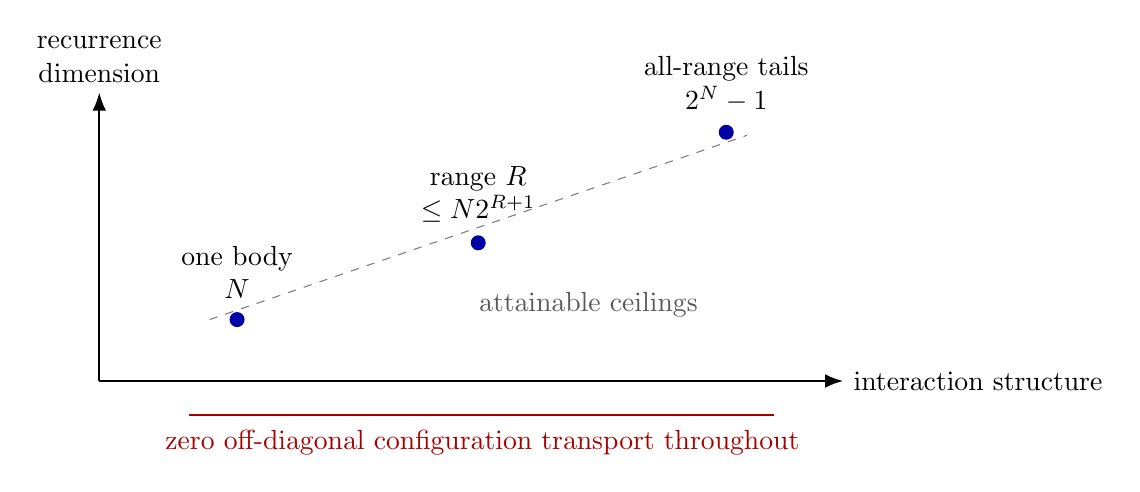
\begin{tikzpicture}[x=1.75cm,y=0.78cm,>=Latex]
  \draw[->,thick] (0,0) -- (5.4,0)
    node[right]{interaction structure};
  \draw[->,thick] (0,0) -- (0,4.7)
    node[above,align=center]{recurrence\\dimension};
  \draw[dashed,gray] (0.8,1.0) -- (4.7,4.0);
  \filldraw[blue!65!black] (1,1) circle (2.5pt);
  \node[above=4pt,align=center] at (1,1)
    {one body\\\(N\)};
  \filldraw[blue!65!black] (2.75,2.25) circle (2.5pt);
  \node[above=4pt,align=center] at (2.75,2.25)
    {range \(R\)\\\(\le N2^{R+1}\)};
  \filldraw[blue!65!black] (4.55,4.05) circle (2.5pt);
  \node[above=4pt,align=center] at (4.55,4.05)
    {all-range tails\\\(2^N-1\)};
  \node[text=gray!70!black] at (3.55,1.25)
    {attainable ceilings};
  \draw[red!65!black,thick] (0.65,-0.55) -- (4.9,-0.55);
  \node[below=2pt,align=center,text=red!65!black] at (2.78,-0.55)
    {zero off-diagonal configuration transport throughout};
\end{tikzpicture}
\caption{\textbf{Spatial support and recurrence arithmetic are independent
coordinates.} Displayed values are attainable ceilings inside the
commuting diagonal l-bit class, not a universal monotone phase diagram.
Fixed range bounds the number of available coefficients; summable all-range
tails can fill the complete projective capacity.}
\label{fig:capacity}
\end{figure}

\section{When interaction layers become visible}

Exact rational rank describes the completed phase orbit and is necessarily
an infinite-precision invariant. A scale-resolved law identifies how its
directions are released.

Assign each support a birth order \(w(S)\in\N\), and consider the polynomial
family
\begin{equation}
 E_g(x)=\sum_{S\subseteq I}g^{w(S)}J_S\chi_S(x).
 \label{eq:scaled}
\end{equation}
Let \(\tau_r\) be the rational rank of all projective spectral jets of
orders \(0,\ldots,r-1\).

\begin{theorem}[Layer-additive temporal dimension]
For every birth-order function, every coefficient family and every
resolution \(r\),
\begin{equation}
 \boxed{
 \tau_r=
 \sum_{m<r}
 \dim_{\Q}\spanQ
 \{J_S:S\ne\varnothing,\ w(S)=m\}.}
 \label{eq:layer}
\end{equation}
No rational independence between different birth layers is required. If
each layer is internally independent, then \(\tau_r\) is the number of
supports with \(w(S)<r\).
\end{theorem}

Distinct birth layers occupy distinct jet coordinates, which is why
cross-layer rational relations do not reduce \(\tau_r\). For birth order
equal to support diameter on \(n\) sites,
\begin{equation}
 \tau_r\le n\,2^{r+1}.
 \label{eq:layergeometry}
\end{equation}
At every fixed resolution, the dimension is therefore linear in system
size even though the completed dimension may be exponential.

The jet law has an exact elapsed-time realization. Every nonempty support
\(S\) defines the balanced integer character \(k_S(x)=\chi_S(x)\). Its
detuning is
\begin{equation}
 \Delta_S(g)=\sum_x k_S(x)E_g(x)
 =2^N J_Sg^{w(S)}.
 \label{eq:detuning}
\end{equation}
Uniformly averaging the phase over the centered time window \([-T,T]\)
gives the exact Fourier reporter
\begin{equation}
 W_S(g,T)=\sinc\!\left(T\Delta_S(g)\right),
 \qquad
 \sinc z=
 \begin{cases}\sin z/z,&z\ne0,\\1,&z=0.\end{cases}
 \label{eq:reporter}
\end{equation}
At the birth horizon \(T=\tau g^{-w(S)}\),
\begin{equation}
 \boxed{
 W_S(g,\tau g^{-w(S)})
 =\sinc(\tau\,2^NJ_S)}
 \label{eq:birth}
\end{equation}
for every \(g\ne0\). For \(J_S\ne0\) and \(\tau>0\), taking
\(g\downarrow0\) at
\(T=\tau g^{-r}\) yields exactly three regimes:
\begin{equation}
 W_S\longrightarrow
 \begin{cases}
  1,&r<w(S),\\
  \sinc(\tau\,2^NJ_S),&r=w(S),\\
  0,&r>w(S).
 \end{cases}
 \label{eq:wall}
\end{equation}
Equations \eqref{eq:layer} and \eqref{eq:wall} connect the algebraic
dimension staircase to elapsed time in the ideal scaled diagonal family.
The qualitative inverse-interaction time scale is known from l-bit
dephasing and revival studies
\cite{HuseNandkishoreOganesyan2014,VasseurParameswaranMoore2015}.
The exact contribution here is the support-by-support
relation--rank--phase-law identity.

\section{One product state sees every direction}

A Hamiltonian can contain spectral directions that a state never samples.
The l-bit result is not hidden in this way. Define the normalized uniform
product state by
\begin{equation}
 \psi_+(x)=2^{-N/2}.
 \label{eq:plus}
\end{equation}
Every configuration has positive Born weight, and its survival amplitude is
\begin{equation}
 A_+(t)=
 \langle\psi_+,\mathrm e^{\,itH_J}\psi_+\rangle
 =2^{-N}\sum_x\mathrm e^{\,itE_J(x)}.
 \label{eq:survival}
\end{equation}

\begin{theorem}[Uniform-state visibility]
The rational gap space visible to \(\psi_+\) equals \(V_{E_J}\).
Consequently its visible temporal dimension is exactly \(\tau(E_J)\).
Moreover, \(\tau(E_J)=2^N-1\) if and only if every completed long-time
survival-fidelity moment of this state attains its unavoidable permutation
collision floor.
\end{theorem}

Thus one explicit state sees the exponential phase rank. The theorem does
not assert that every local observable can reconstruct it efficiently, nor
that the l-bit product state is easy to prepare when the microscopic
dressing unitary is unknown.

\section{An infinite quasi-local sharpness construction}

Finite-window maximality is compatible with one genuine infinite energy
law. There exists one coefficient assignment on every nonempty finite
support \(S\subset\N\) such that
\begin{equation}
 \sum_S|J_S|<\infty,\qquad
 |J_S|\le
 2^{-\left(|S|+\max S+\operatorname{diam}S\right)},
 \label{eq:envelope}
\end{equation}
and every finite subfamily is rationally independent. Therefore every
finite embedded window \(\Lambda\) has
\begin{equation}
 \tau(E_{J|\Lambda})=2^{|\Lambda|}-1.
 \label{eq:allwindows}
\end{equation}

For every infinite Boolean configuration \(\sigma\), the series
\begin{equation}
 E_\infty(\sigma)=\sum_SJ_S\chi_S(\sigma)
 \label{eq:infiniteenergy}
\end{equation}
converges absolutely. It is bounded and continuous in the product topology,
and its nested first-\(n\)-site truncations converge uniformly with error
bounded by the omitted absolute interaction mass.

On the Banach space of continuous complex amplitudes, it generates
\begin{equation}
 (U_t\psi)(\sigma)=
 \exp\!\left(-itE_\infty(\sigma)\right)\psi(\sigma),
 \label{eq:evolution}
\end{equation}
a reversible strongly continuous group of complex-linear isometries in the
uniform norm.

For a site \(x\), let \(X_x\) flip the Boolean coordinate \(x\), and set
\(\tau_t(X_x)=U_tX_xU_{-t}\). The diameter-weighted interaction mass
\begin{equation}
 K=\sum_S2^{\operatorname{diam}S}|J_S|
 \label{eq:weightedmass}
\end{equation}
is finite. For every pair of sites, every time and every continuous
amplitude,
\begin{equation}
 \bigl\|[\tau_t(X_x),X_y]\psi\bigr\|_\infty
 \le
 \min\!\left\{2,\,
 4K|t|\,2^{-|x-y|}\right\}\|\psi\|_\infty .
 \label{eq:influencecone}
\end{equation}
Yet if \(F\) is any finite environment not containing \(x\), the complete
packet of conditional frequencies of the same flip has
\begin{equation}
 \tau_x(F)=2^{|F|}.
 \label{eq:localfliprank}
\end{equation}

Let \(\mathcal C_{xy}(t)\) denote the induced uniform-norm size of this
commutator,
\[
 \mathcal C_{xy}(t)=
 \sup_{\|\psi\|_\infty=1}
 \bigl\|[\tau_t(X_x),X_y]\psi\bigr\|_\infty .
\]

\begin{theorem}[Delayed all-pairs influence saturation]
For every two distinct sites \(x,y\), there is an explicit \(t_{xy}>0\)
such that
\begin{equation}
 \boxed{\mathcal C_{xy}(t_{xy})=
 \sup_{t\in\R}\mathcal C_{xy}(t)=2.}
 \label{eq:allsaturation}
\end{equation}
The same fixed-time locality bound forces
\begin{equation}
 \boxed{
 2\le
 4K t_{xy}2^{-|x-y|}.}
 \label{eq:saturationdelay}
\end{equation}
\end{theorem}

Thus no pair is permanently isolated, but maximal influence cannot occur
before paying an exponentially growing distance factor. The upper and
lower conclusions concern exactly the same coefficient field and the same
two local flips. At the all-false configuration, the double-flip energy
difference is
\[
 4\sum_{S\ni x,y}J_S>0.
\]
Choosing \(t_{xy}\) as its inverse half-period makes the two phases
antipodal and saturates the universal two-unit ceiling.

There is also an exact same-packet law connecting spatial cost to the
conditional recurrence dimension it creates. Fix the flip at site \(0\),
let \(F_r=\{1,\ldots,r\}\), set \(y_r=r+1\) and \(D_r=2^r\), and define the
boundary-born packet
\begin{equation}
 b_{r,S}=J_{\{0,y_r\}\cup S},
 \qquad S\subseteq F_r.
 \label{eq:boundarypacket}
\end{equation}

\begin{theorem}[Boundary recurrence--locality budget]
Resolving \(y_r\) doubles the exact conditional frequency rank:
\begin{equation}
 \boxed{\tau_0(F_r)=D_r,\qquad
 \tau_0(F_r\cup\{y_r\})=2D_r.}
 \label{eq:boundarydoubling}
\end{equation}
The new half consists exactly of the \(D_r\) rationally independent
coefficients in \eqref{eq:boundarypacket}, and the same packet obeys
\begin{equation}
 \boxed{
 2D_r\sum_{S\subseteq F_r}|b_{r,S}|\le K.}
 \label{eq:boundarymass}
\end{equation}
For \(\delta>0\), let
\(N_{r,\delta}=|\{S\subseteq F_r:|b_{r,S}|\ge\delta\}|\). Then
\begin{equation}
 \boxed{
 2D_r\delta N_{r,\delta}\le K.}
 \label{eq:boundarythreshold}
\end{equation}
In particular, resolving all \(D_r\) new coefficients above the same
threshold forces
\begin{equation}
 \boxed{2\delta D_r^2\le K.}
 \label{eq:boundaryquadratic}
\end{equation}
\end{theorem}

Equations \eqref{eq:influencecone}, \eqref{eq:localfliprank},
\eqref{eq:allsaturation} and \eqref{eq:boundaryquadratic} form one
same-field infinite law. At fixed time, influence is exponentially
suppressed outside a logarithmic light cone. Over all time, every pair
attains maximal influence. Each additional resolved boundary site doubles
the exact conditional clock dimension, while the same coefficients pay a
quadratic full-resolution locality budget.

This construction proves that absolute summability and the explicit
origin-dependent exponential envelope \eqref{eq:envelope} do not impose
the finite-range ceiling. It is not a claim of a global exact recurrence,
a selected \(L^2\) quantum representation, translation invariance, or a
derivation from a microscopic random-field Hamiltonian. The threshold
\(\delta\) in \eqref{eq:boundarythreshold} is a coefficient threshold, not
a theorem about detector noise or finite-time statistical
distinguishability.

\section{Localization compresses the recurrence clock seen at one site}

The global rank \(\tau(E)\) is not the clock dimension seen by every
observer. Let a normalized state localized at a site \(x\) have Born
weights \(p_k(x)\) in a finite pure-point eigenbasis, and write
\[
 S_x(t)=
 \left|\sum_k p_k(x)e^{-itE_k}\right|^2
\]
for its survival probability. Assign to mode \(k\) a centre at integer
distance \(r_k\) from \(x\). Suppose, for explicit constants,
\begin{equation}
 p_k(x)\le C e^{-2\mu r_k},\qquad
 \#\{k:r_k=m\}\le AB^m,\qquad
 q:=Be^{-2\mu}<1 .
 \label{eq:localizationcertificate}
\end{equation}
For the modes inside radius \(R\), put
\[
 S_R=\{k:r_k\le R\},\qquad
 \beta_R=AC\frac{q^{R+1}}{1-q}.
\]

\begin{theorem}[Observer-localized recurrence]
\label{thm:observer-localized-recurrence}
If \(S_R\ne\varnothing\), then for every integer phase resolution
\(Q\ge0\) there is a positive integer \(n\) such that
\begin{equation}
 n\le(Q+1)^{|S_R|-1},\qquad
 1-S_x(n)\le
 4\beta_R+
 2\left(\frac{2\pi}{Q+1}\right)^2 .
 \label{eq:localized-return}
\end{equation}
Consequently, if \(|S_R|\le V_{\rm eff}(R)\), the ambient spectral
dimension in the deadline can be replaced by \(V_{\rm eff}(R)\). At the
same budget there is an exhaustive alternative: the survival history never
leaves the certified neighborhood, or an exit is followed strictly later
by a return within the same localization-volume deadline.
\end{theorem}

The first term in \eqref{eq:localized-return} is the total loss caused by
discarding the localized spectral tail. The second is the squared
phase-synchronization error of the retained modes. The exponent
\(|S_R|-1\) is their projective phase capacity. Thus localization does
more than inhibit transport: it bounds how much of the global recurrence
torus a site-local survival history must synchronize.

Finiteness of the spectrum is not essential. For a normalized nonnegative
countable pure-point packet, retain a head of \(M\ge1\) modes and certify
tail mass at most \(\alpha\). Then some positive integer \(n\) obeys
\begin{equation}
 n\le(Q+1)^{M-1},\qquad
 1-S_x(n)\le
 \left(\frac{2\pi}{Q+1}\right)^2
 \sum_{k=1}^{M-1}p_k(x)+4\alpha ,
 \label{eq:countable-localized-return}
\end{equation}
with the same never-exits/post-exit-return alternative. Countable ambient
support therefore enters only through the certified tail; the visible head
sets the return exponent.

Equations \eqref{eq:localized-return} and
\eqref{eq:countable-localized-return} are deterministic interfaces. They
apply whenever the explicit eigensystem certificate
\eqref{eq:localizationcertificate}, or its countable tail analogue, has
been established. They do not assert that every random Hamiltonian is
localized. Their relevance to Anderson theory is precise: a
model-specific localization theorem supplies the spectral tail, and the
recurrence law converts that spatial certificate into a local temporal
deadline.

\section{Anderson locality is an order of quantifiers}

Anderson dynamical localization asks for spatial decay after taking the
supremum over all times. In the equivalent spin-language formulation this
appears as a zero-velocity Lieb--Robinson bound; such a bound is known for
the random-field isotropic XY chain
\cite{HamzaSimsStolz2012}. Equation \eqref{eq:influencecone} instead takes
distance to infinity at fixed \(t\). Equation \eqref{eq:allsaturation}
proves that the order cannot be reversed for the interacting field:
\begin{equation}
 \boxed{
 \text{fixed-time exponential locality}
 \ \not\Rightarrow\
 \text{time-uniform Anderson locality}.}
 \label{eq:quantifierseparation}
\end{equation}
Indeed, its all-time commutator envelope is exactly \(2\) for every
distinct pair, independent of distance. This is a classification of the
constructed dynamics, not a claim that the field is Anderson localized.

The exact connection to Anderson physics is an endpoint, not an identity of
the two theories. Diagonalizing a noninteracting fermionic Hamiltonian gives
\[
 H_{\mathrm F}=\sum_{j=1}^{N}\varepsilon_j n_j.
\]
Its complete Fock spectrum contains only the \(N\) one-particle energies as
rational generators, so \(\tau\le N\), with equality when the
\(\varepsilon_j\) are rationally independent. Anderson localization can
make the corresponding orbitals spatially localized, but localization is
irrelevant to this algebraic bound.

A finite Anderson matrix gives a complementary exact separation without
assuming an l-bit representation. Let \(T\) be any \(N\times N\) Hermitian
hopping matrix and
\[
H_p=T+\operatorname{diag}(p_1,\ldots,p_N).
\]

\begin{theorem}[Finite Anderson all-time spatial separation]
\label{thm:anderson-separation}
For every \(N>0\), every Hermitian \(T\), every metric \(d\) on the sites
and every \(C,\mu>0\), there is an onsite potential \(p\in\R^N\) such that
\[
 \dim_{\Q}\spanQ\{E_j-E_1:2\le j\le N\}=N-1
 \label{eq:anderson-fullrank}
\]
for the eigenvalues of \(H_p\), while simultaneously
\[
 \left|\langle i|\exp(-itH_p)|j\rangle\right|
 < C e^{-\mu d(i,j)}
 \quad\text{for every }i\ne j
 \text{ and every }t\in\R .
 \label{eq:anderson-nonexit}
\]
For every reference level, completed sampling of the relative phases
converges to Haar probability on the full \((N-1)\)-torus.
\end{theorem}

Thus a fixed-hopping Hamiltonian can have the largest possible global
recurrence dimension while every site-to-site transition obeys any
prescribed positive finite spatial envelope for unbounded time. The proof
resolves the spectrum into separated clusters near the atomic limit; the
cluster-projector mixing budget is time independent and bounds the
propagator for all \(t\). A global energy and time rescaling converts the
near-atomic construction to fixed hopping, with the onsite disorder
rescaled instead. This is a finite-dimensional all-time theorem. The
required onsite scale, and hence the exponential envelope, need not be
uniform in system size. The theorem is therefore not a thermodynamic-limit
localization statement or a probability estimate for a named disorder
ensemble. Its role is to show that spatial confinement can hide a maximal
global recurrence clock without destroying it, already inside the
ordinary finite onsite-plus-hopping family rather than only at the
diagonal l-bit endpoint.

Interactions between localized conserved modes generate the higher-support
coefficients \(J_S\) in \eqref{eq:lbit}. The dimension law then determines
exactly how many free-Fock relations they remove. This explains why
interaction-induced dephasing can strongly suppress revivals while
configuration transport remains absent. It does not claim the first
observation of that suppression
\cite{VasseurParameswaranMoore2015}, nor does it claim that a generic
microscopic many-body localized Hamiltonian has maximal rank.

The latter transfer is a distinct open technical boundary. A standard
random-field XXZ or Anderson--Hubbard Hamiltonian has a narrow, correlated
parameter family; an abstract full-rank l-bit coefficient assignment does
not prove that its microscopic spectrum avoids every balanced integer
relation while localization persists. Imbrie's rigorous l-bit
diagonalization also carries an explicit level-attraction assumption
\cite{Imbrie2016}. Theorems \eqref{eq:lbitrank}--\eqref{eq:wall} apply
exactly once the diagonal l-bit energy law is given; they do not derive that
law for a microscopic ensemble.

\section{Discussion}

The universal law is the projective conservation budget
\(\tau(E)+\dim_\Q L_E^{\mathrm{proj}}=D-1\) for every finite spectrum.
Its localization consequence is a threefold separation:
\begin{equation}
 \boxed{
 \begin{gathered}
 \text{configuration transport can vanish while recurrence dimension is
 maximal},\\
 \text{a local recurrence deadline can depend on localization volume
 rather than ambient dimension},\\
 \text{fixed-time exponential locality can coexist with maximal eventual
 all-pairs influence}.
 \end{gathered}}
 \label{eq:separation}
\end{equation}
The second line is precisely where interacting quasi-local dynamics parts
company with time-uniform Anderson dynamical localization. The boundary law
then identifies a cost within the same mechanism: one added site doubles
the exact conditional recurrence dimension, but complete coefficient-level
resolution of the new \(D\)-dimensional packet consumes at least
\(2\delta D^2\) of the diameter-weighted locality budget.

The law also reorganizes quantitative recurrence results. Once
\(\tau(E)\) is known, return-time bounds concern approximation inside a
\(\tau(E)\)-dimensional compact phase orbit rather than the raw Hilbert
dimension. Observer restrictions replace that orbit by a quotient.
Replica depth filters its integer annihilator. Weak interactions can leave
all bounded-time dynamics close while changing the completed orbit
dimension discontinuously. These are not separate recurrence mechanisms;
they are geometric and operational shadows of
\eqref{eq:universal}.

Three earlier recurrence laws now acquire a common position in this
geometry. For a weighted finite packet, the logarithm of the least
worst-spectrum return deadline and the negative logarithm of the exact
return-target volume are controlled, within explicit support-linear
constants, by the same pivot-optimized reverse-water information; this is
target geometry inside the completed phase orbit. For a finite family of
operator probes, the coherence graph gives class-wide visible capacity
\(d-c(G)\), after which the actual spectral relation lattice can only reduce
the dimension; this is an observer quotient. For an arbitrary probability
spectrum, every completed survival-fidelity moment is the zero-sum
collision probability of independent visible energy gaps; this is a scalar
pushforward of the completed phase law. The localization results determine
the parent orbit on which all three constructions act.

The logarithmic light cone, l-bit spectral tree and interaction-induced OTO
dephasing are established results
\cite{KimChandranAbanin2014,NandkishoreGopalakrishnanHuse2014,
ChenZhouHuseFradkin2017}. The exact contribution here is not their
rediscovery. It is the rational relation classification, the all-pairs
saturation theorem, and the same-boundary dimension--mass budget for one
coefficient field, joined to the universal projective conservation law.

The theorem's scope is exact. Rational rank is an infinite-precision
spectral invariant. The threshold law is coefficient-level rather than a
device-noise statement. The infinite construction acts isometrically on
continuous amplitudes in the uniform norm and is not identified with a
chosen \(L^2\) representation. The finite fixed-hopping theorem is
all-time but not volume-uniform. No statement is made about a generic
random-field XXZ or Anderson--Hubbard ensemble. Within that scope, spatial
geometry constrains where interaction coordinates can live; recurrence
arithmetic determines how many projective phases remain; and the
all-time supremum distinguishes permanent Anderson confinement from
exponentially delayed interacting influence.

\section{Methods}

\subsection{Projective detuning and rank--nullity}

Let
\[
 \mathcal Q_X=\{q\in\Q^X:\sum_xq_x=0\}.
\]
The projective detuning map
\[
 D_E:\mathcal Q_X\to\R,\qquad
 D_E(q)=\sum_xq_xE(x)
\]
has kernel \(L_E^{\mathrm{proj}}\). Its image is exactly the anchored gap
space \(V_E\): elementary difference characters generate every anchored
gap, while the zero-charge condition rewrites every detuning as a rational
combination of such gaps. Since
\(\dim_{\Q}\mathcal Q_X=D-1\), rank--nullity gives
\eqref{eq:universal}.

\subsection{Walsh extraction}

For Boolean configurations,
\[
 \sum_x\chi_S(x)\chi_T(x)=2^N\mathbf 1_{S=T}.
\]
Applying this identity to \eqref{eq:lbit} gives
\[
 \sum_x\chi_S(x)E_J(x)=2^NJ_S.
\]
Every \(J_S\) is therefore in the rational span of the energies, whereas
the Walsh expansion puts every energy in the span of the \(J_S\). Removing
the constant coefficient proves \eqref{eq:lbitrank}. The same extraction
with coefficients \(g^{w(S)}J_S\) proves \eqref{eq:detuning}.

\subsection{Finite-time phase reporter}

For a real detuning \(\Delta\), normalized centered averaging gives
\[
 \frac{1}{2T}\int_{-T}^{T}\mathrm e^{it\Delta}\,dt
 =\sinc(T\Delta).
\]
Substitution of \eqref{eq:detuning} proves
\eqref{eq:reporter} and the exact cancellation of powers in
\eqref{eq:birth}. The three limits in \eqref{eq:wall} follow from continuity
of sinc at zero and its decay at infinity.

\subsection{Geometric support counting}

The rank of a coefficient packet cannot exceed its cardinality. A support
of diameter at most \(R\) is contained in a window of at most \(R+1\)
ordered sites. Assigning each support to a possible left endpoint and then
counting subsets gives
\(|\mathcal S_{n,R}|\le n2^{R+1}\). Rational independence of the allowed
coefficient packet attains the intrinsic support-count ceiling.

\subsection{Infinite construction}

Assign each nonempty finite support a distinct prime logarithm and multiply
it by a nonzero rational dyadic scale. The scale penalizes an injective
support encoding, support cardinality, rightmost extent and diameter.
Rational independence of distinct prime logarithms survives the rescaling,
while the encoding term supplies a summable geometric majorant and implies
\eqref{eq:envelope}. Absolute summability gives uniform convergence of
\eqref{eq:infiniteenergy}; finite-support Walsh characters are continuous,
so the uniform limit is continuous. Multiplication by the unit-modulus
phase in \eqref{eq:evolution} gives the group law, inverse, norm
preservation and strong continuity. A double flip at \(x,y\) cancels every
interaction support not containing both sites. Each surviving term costs
at most \(4|J_S|\), while \(x,y\in S\) implies
\(|x-y|\le\operatorname{diam}S\). Summing against
\eqref{eq:weightedmass} gives the factor \(4K2^{-|x-y|}\). The unitary
phase is Lipschitz in its real generator with constant \(|t|\), yielding
\eqref{eq:influencecone}; the universal bound \(2\) follows from the
triangle inequality. Finally, supports \(S\subseteq F\) map injectively to
the incident supports \(S\cup\{x\}\). Rational independence survives this
restriction, and finite Walsh inversion gives \eqref{eq:localfliprank}.

All nonempty coefficients in the explicit field are positive. At the
all-false configuration this gives the strictly positive double-flip
detuning
\[
 \Delta_{xy}=4\sum_{S\ni x,y}J_S.
\]
At \(t_{xy}=\pi/\Delta_{xy}\), the two Heisenberg flip phases are antipodal.
The constant unit amplitude therefore witnesses
\(\mathcal C_{xy}(t_{xy})=2\), while the universal triangle bound gives
\(\mathcal C_{xy}(t)\le2\) at every time. Substituting this equality into
\eqref{eq:influencecone} proves \eqref{eq:saturationdelay}.

For the boundary law, the map
\[
 S\subseteq F_r\longmapsto \{0,r+1\}\cup S
\]
is injective and every image support has diameter at least \(r+1\).
Rational independence of the global coefficient field therefore makes the
\(D_r=2^r\) boundary packet independent. Finite Walsh inversion identifies
it with exactly the new half of the conditional frequency packet, proving
\eqref{eq:boundarydoubling}. Its contribution to the weighted mass is at
least
\[
 2^{r+1}\sum_{S\subseteq F_r}|b_{r,S}|
 =2D_r\sum_{S\subseteq F_r}|b_{r,S}|,
\]
which proves \eqref{eq:boundarymass}. Restricting the sum to coefficients
of magnitude at least \(\delta\) proves
\eqref{eq:boundarythreshold}; setting \(N_{r,\delta}=D_r\) gives
\eqref{eq:boundaryquadratic}.

\section*{Data availability}

No datasets were generated or analysed in this theoretical study.

\section*{Competing interests}

The author declares no competing interests.

\section*{Use of generative artificial intelligence}

Generative language models assisted literature triage, proof exploration
and draft preparation. The human author takes responsibility for the
manuscript, mathematical arguments, citations and conclusions.

\begin{thebibliography}{99}
\small
\raggedright

\bibitem{Anderson1958}
P.~W.~Anderson,
Absence of diffusion in certain random lattices,
\emph{Phys. Rev.} \textbf{109}, 1492--1505 (1958).
\href{https://doi.org/10.1103/PhysRev.109.1492}
{doi:10.1103/PhysRev.109.1492}.

\bibitem{SerbynPapicAbanin2013}
M.~Serbyn, Z.~Papi\'c and D.~A.~Abanin,
Local conservation laws and the structure of the many-body localized
states,
\emph{Phys. Rev. Lett.} \textbf{111}, 127201 (2013).
\href{https://arxiv.org/abs/1305.5554}{arXiv:1305.5554}.

\bibitem{HuseNandkishoreOganesyan2014}
D.~A.~Huse, R.~Nandkishore and V.~Oganesyan,
Phenomenology of fully many-body-localized systems,
\emph{Phys. Rev. B} \textbf{90}, 174202 (2014).
\href{https://arxiv.org/abs/1408.4297}{arXiv:1408.4297}.

\bibitem{KimChandranAbanin2014}
I.~H.~Kim, A.~Chandran and D.~A.~Abanin,
Local integrals of motion and the logarithmic lightcone in many-body
localized systems,
\href{https://arxiv.org/abs/1412.3073}{arXiv:1412.3073} (2014).

\bibitem{NandkishoreGopalakrishnanHuse2014}
R.~Nandkishore, S.~Gopalakrishnan and D.~A.~Huse,
Spectral features of a many-body-localized system weakly coupled to a heat
bath,
\emph{Phys. Rev. B} \textbf{90}, 064203 (2014).
\href{https://doi.org/10.1103/PhysRevB.90.064203}
{doi:10.1103/PhysRevB.90.064203}.

\bibitem{ChenZhouHuseFradkin2017}
X.~Chen, T.~Zhou, D.~A.~Huse and E.~Fradkin,
Out-of-time-order correlations in many-body localized and thermal phases,
\emph{Ann. Phys. (Berlin)} \textbf{529}, 1600332 (2017).
\href{https://doi.org/10.1002/andp.201600332}
{doi:10.1002/andp.201600332}.

\bibitem{HamzaSimsStolz2012}
E.~Hamza, R.~Sims and G.~Stolz,
Dynamical localization in disordered quantum spin systems,
\emph{Commun. Math. Phys.} \textbf{315}, 215--239 (2012).
\href{https://doi.org/10.1007/s00220-012-1544-6}
{doi:10.1007/s00220-012-1544-6}.

\bibitem{VasseurParameswaranMoore2015}
R.~Vasseur, S.~A.~Parameswaran and J.~E.~Moore,
Quantum revivals and many-body localization,
\emph{Phys. Rev. B} \textbf{91}, 140202(R) (2015).
\href{https://arxiv.org/abs/1407.4476}{arXiv:1407.4476}.

\bibitem{Imbrie2016}
J.~Z.~Imbrie,
On many-body localization for quantum spin chains,
\emph{J. Stat. Phys.} \textbf{163}, 998--1048 (2016).
\href{https://arxiv.org/abs/1403.7837}{arXiv:1403.7837}.

\bibitem{RiddellPagliaroliAlhambra2023}
J.~Riddell, N.~J.~Pagliaroli and A.~M.~Alhambra,
Concentration of quantum equilibration and an estimate of the recurrence
time,
\emph{SciPost Phys.} \textbf{15}, 165 (2023).
\href{https://arxiv.org/abs/2206.07541}{arXiv:2206.07541}.

\bibitem{RiddellBertini2024}
J.~Riddell and B.~Bertini,
Rationally independent free fermions with local hopping,
\href{https://arxiv.org/abs/2404.12100}{arXiv:2404.12100} (2024).

\end{thebibliography}

\end{document}
